

\begin{center}
\thispagestyle{empty}
%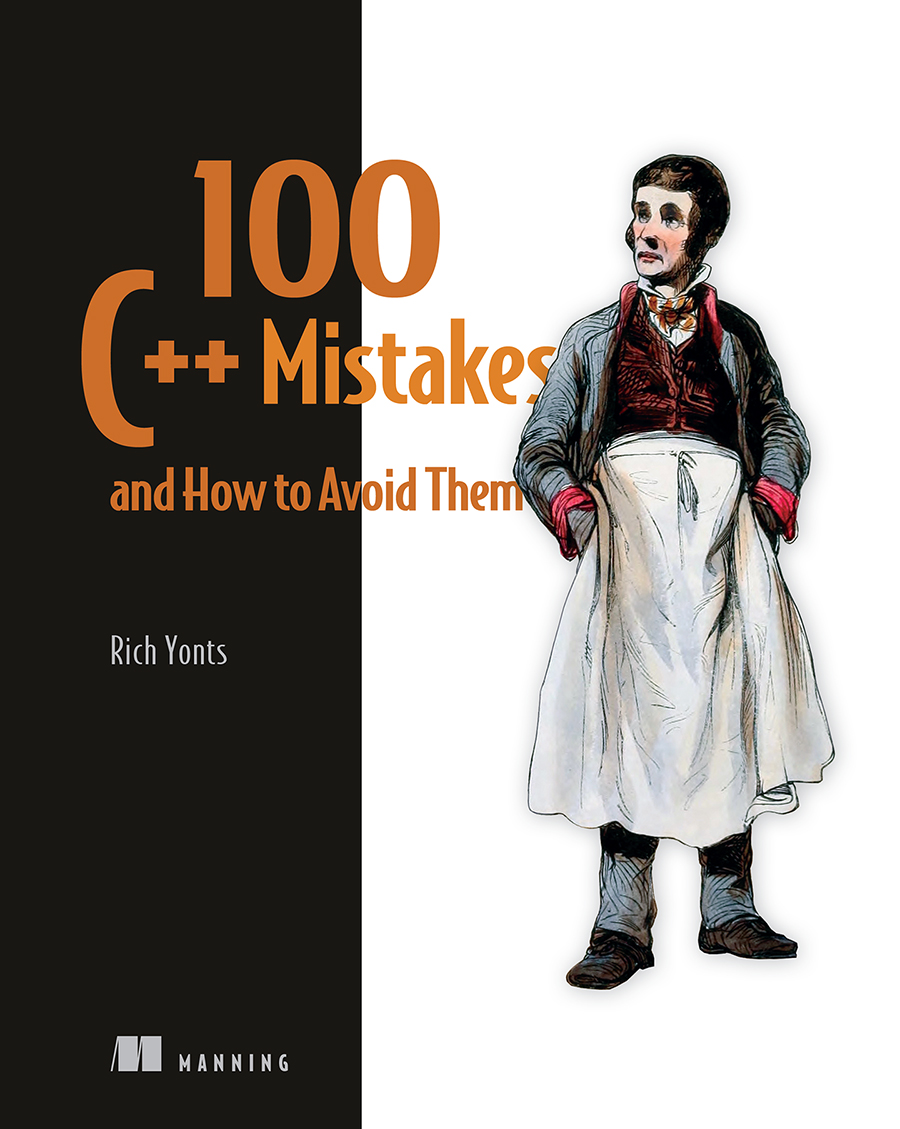
\includegraphics[width=\textwidth,height=\textheight,keepaspectratio]{cover.png}
\begin{tikzpicture}[remember picture, overlay, inner sep=0pt]
\node at (current page.center)
{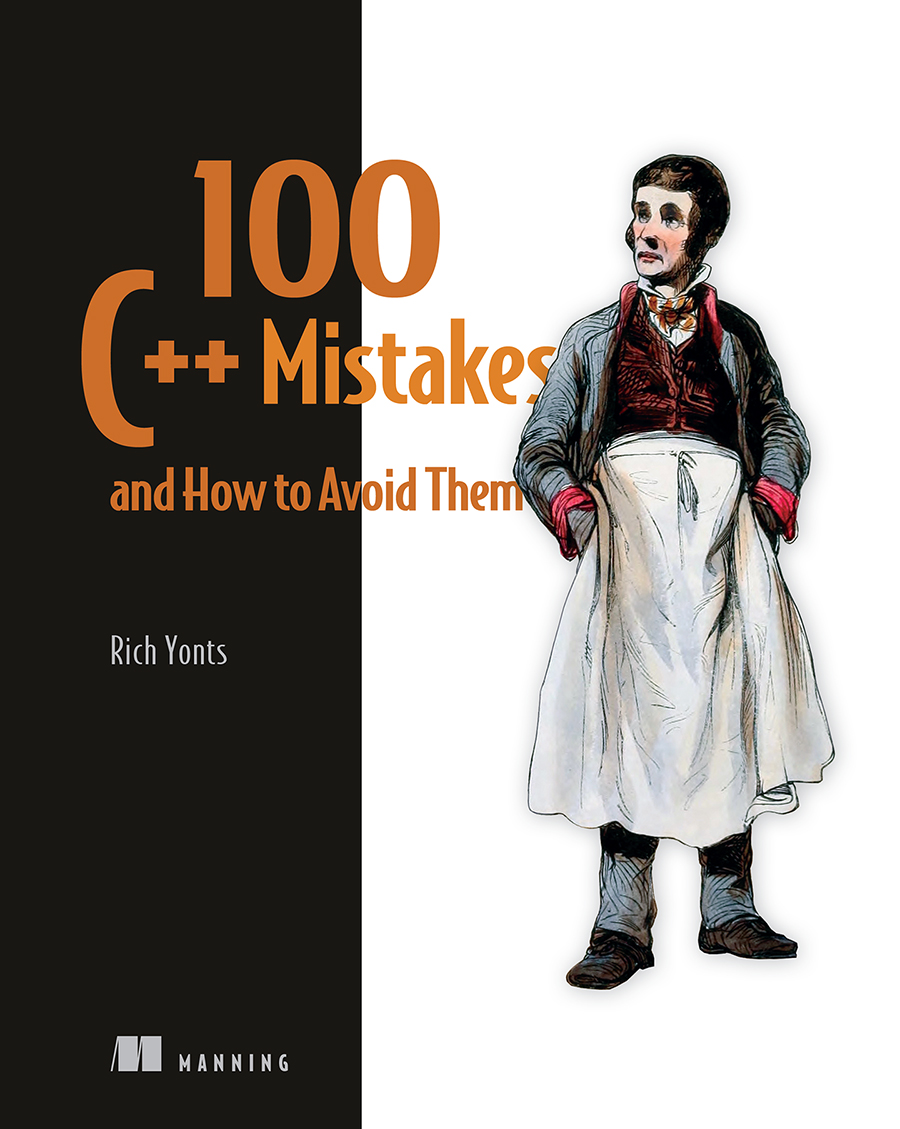
\includegraphics[width=\paperwidth, keepaspectratio=false]{cover.png}};
\end{tikzpicture}
\newpage
\thispagestyle{empty}
\huge
\textbf{C++编程避坑指南:100个常见错误及解决方案}
\\[9pt]
\normalsize
作者: Rich Yonts
\\[8pt]
\normalsize
译者:\href{https://github.com/xiaoweiChen/100-Cpp-Mistakes-and-How-to-Avoid-Them}{陈晓伟}
\\[8pt]
\end{center}

\newpage

\begin{comment}
\end{comment}

\myChapterNoContents{前言}{}{content/preface.tex}
\newpage

\myChapterNoContents{致谢}{}{content/acknowledgments.tex}
\newpage

\myChapterNoContents{关于本书}{}{content/about-this-book.tex}
\newpage

\myChapterNoContents{关于作者}{}{content/about-the-author.tex}
\newpage

\myChapterNoContents{封面插图}{}{content/about-the-cover-illustration.tex}
\newpage

\pagestyle{empty}
\tableofcontents
\newpage

\setsecnumdepth{section}

\myChapter{第1章}{C++: With great power comes great responsibility}{content/chapter1/0.tex}
\mySubsection{1.1.}{Mistakes}{content/chapter1/1.tex}
\mySubsection{1.2.}{Anatomy of a mistake}{content/chapter1/2.tex}
\mySubsection{1.3.}{Learning from our mistakes}{content/chapter1/3.tex}
\mySubsection{1.4.}{Where we’ll find mistakes}{content/chapter1/4.tex}
\mySubsection{1.5.}{A word about organization}{content/chapter1/5.tex}
\mySubsection{1.6.}{总结}{content/chapter1/6.tex}
\newpage

\myPartGray{第一部分}{现代 C++}{content/part1/part.tex}
\newpage

\myChapter{第2章}{Better modern C++: Classes and types}{content/part1/chapter2/0.tex}
\mySubsection{2.1.}{Mistake 1: Failing to use move semantics}{content/part1/chapter2/1.tex}
\mySubsection{2.2.}{Mistake 2: Using empty exception specifications}{content/part1/chapter2/2.tex}
\mySubsection{2.3.}{Mistake 3: Not using override on derived virtual functions}{content/part1/chapter2/3.tex}
\mySubsection{2.4.}{Mistake 4: Writing simple or hiding unwanted supplied class members}{content/part1/chapter2/4.tex}
\mySubsection{2.5.}{Mistake 5: Not using in-class initializers}{content/part1/chapter2/5.tex}
\mySubsection{2.6.}{Mistake 6: Overusing index-based loops}{content/part1/chapter2/6.tex}
\mySubsection{2.7.}{Mistake 7: Failing to use nullptr}{content/part1/chapter2/7.tex}
\mySubsection{2.8.}{Mistake 8: Not using unique\_ptrs for exclusive ownership}{content/part1/chapter2/8.tex}
\mySubsection{2.9.}{Mistake 9: Not using shared\_ptrs for shared ownership}{content/part1/chapter2/9.tex}
\newpage

\myChapter{第3章}{Better modern C++: General programming}{content/part1/chapter3/0.tex}
\mySubsection{3.1.}{Mistake 10: Failing to use if with initialization}{content/part1/chapter3/1.tex}
\mySubsection{3.2.}{Mistake 11: Not using type inference for variables}{content/part1/chapter3/2.tex}
\mySubsection{3.3.}{Mistake 12: Using typedef}{content/part1/chapter3/3.tex}
\mySubsection{3.4.}{Mistake 13: Writing common algorithms}{content/part1/chapter3/4.tex}
\mySubsection{3.5.}{Mistake 14: Not using uniform initialization}{content/part1/chapter3/5.tex}
\mySubsection{3.6.}{Mistake 15: Failing to use emplacement}{content/part1/chapter3/6.tex}
\mySubsection{3.7.}{Mistake 16: Failing to use tuples}{content/part1/chapter3/7.tex}
\mySubsection{3.8.}{Mistake 17: Not using structured binding}{content/part1/chapter3/8.tex}
\newpage

\myChapter{第4章}{Better modern C++: Additional topics}{content/part1/chapter4/0.tex}
\mySubsection{4.1.}{Mistake 18: Not using variadic templates}{content/part1/chapter4/1.tex}
\mySubsection{4.2.}{Mistake 19: Using global namespace enums}{content/part1/chapter4/2.tex}
\mySubsection{4.3.}{Mistake 20: Not using new formatting functionality}{content/part1/chapter4/3.tex}
\mySubsection{4.4.}{Mistake 21: Not using ranges with containers}{content/part1/chapter4/4.tex}
\mySubsection{4.5.}{Mistake 22: Writing nonportable filesystem code}{content/part1/chapter4/5.tex}
\mySubsection{4.6.}{Mistake 23: Writing excessive standalone functions}{content/part1/chapter4/6.tex}
\mySubsection{4.7.}{Mistake 24: Using awkward constants}{content/part1/chapter4/7.tex}
\mySubsection{4.8.}{Mistake 25: Writing pattern-matching code}{content/part1/chapter4/8.tex}
\newpage

\myPartGray{第二部分}{Transitional C++}{content/part2/part.tex}
\newpage

\myChapter{第5章}{C idioms}{content/part2/chapter5/0.tex}
\mySubsection{5.1.}{Mistake 26: Always declaring variables at the top of a function}{content/part2/chapter5/1.tex}
\mySubsection{5.2.}{Mistake 27: Depending on macros}{content/part2/chapter5/2.tex}
\mySubsection{5.3.}{Mistake 28: Misunderstanding NULL}{content/part2/chapter5/3.tex}
\mySubsection{5.4.}{Mistake 29: Accessing disk files using FILE}{content/part2/chapter5/4.tex}
\mySubsection{5.5.}{Mistake 30: Using integers for Boolean values}{content/part2/chapter5/5.tex}
\mySubsection{5.6.}{Mistake 31: Using C-style casts}{content/part2/chapter5/6.tex}
\mySubsection{5.7.}{Mistake 32: Converting text with atoi}{content/part2/chapter5/7.tex}
\mySubsection{5.8.}{Mistake 33: Using C-style strings}{content/part2/chapter5/8.tex}
\mySubsection{5.9.}{Mistake 34: Calling the exit function}{content/part2/chapter5/9.tex}
\mySubsection{5.10.}{Mistake 35: Preferring arrays to vectors}{content/part2/chapter5/10.tex}
\newpage

\myChapter{第6章}{Better premodern C++}{content/part2/chapter6/0.tex}
\mySubsection{6.1.}{Mistake 36: Input and output using scanf and printf}{content/part2/chapter6/1.tex}
\mySubsection{6.2.}{Mistake 37: Overusing endl}{content/part2/chapter6/2.tex}
\mySubsection{6.3.}{Mistake 38: Dynamic allocation with malloc and free}{content/part2/chapter6/3.tex}
\mySubsection{6.4.}{Mistake 39: Using unions for type conversion}{content/part2/chapter6/4.tex}
\mySubsection{6.5.}{Mistake 40: Using varargs for variable parameter lists}{content/part2/chapter6/5.tex}
\mySubsection{6.5.}{Mistake 41: Incorrect class initialization order}{content/part2/chapter6/6.tex}
\mySubsection{6.5.}{Mistake 42: Adding nonvalue types to containers}{content/part2/chapter6/7.tex}
\mySubsection{6.5.}{Mistake 43: Favoring indexes over iterators}{content/part2/chapter6/8.tex}
\newpage

\myPartGray{第三部分}{Classic (premodern) C++}{content/part3/part.tex}
\newpage

\myChapter{第7章}{Establishing the class invariant}{content/part3/chapter7/0.tex}
\mySubsection{7.1.}{Class invariants enforce proper class design}{content/part3/chapter7/1.tex}
\mySubsection{7.2.}{Mistakes in class design}{content/part3/chapter7/2.tex}
\mySubsection{7.3.}{Mistake 44: Failing to maintain the class invariant}{content/part3/chapter7/3.tex}
\mySubsection{7.4.}{Mistake 45: Not thinking of classes as data types}{content/part3/chapter7/4.tex}
\mySubsection{7.5.}{Mistake 46: Not establishing a basis for methods}{content/part3/chapter7/5.tex}
\mySubsection{7.6.}{Mistake 47: Failing to code the big 3}{content/part3/chapter7/6.tex}
\mySubsection{7.7.}{Mistake 48: Using inheritance just for code reuse}{content/part3/chapter7/7.tex}
\mySubsection{7.8.}{Mistake 49: Overusing default constructors}{content/part3/chapter7/8.tex}
\mySubsection{7.9.}{Mistake 50: Failing to maintain the is-a relationship}{content/part3/chapter7/9.tex}
\newpage

\myChapter{第8章}{Maintaining the class invariant}{content/part3/chapter8/0.tex}
\mySubsection{8.1.}{Maintaining the class invariant}{content/part3/chapter8/1.tex}
\mySubsection{8.2.}{Mistake 51: Writing nonessential accessors}{content/part3/chapter8/2.tex}
\mySubsection{8.3.}{Mistake 52: Providing trivial mutators}{content/part3/chapter8/3.tex}
\mySubsection{8.4.}{Mistake 53: Overusing protected instance variables}{content/part3/chapter8/4.tex}
\mySubsection{8.5.}{Mistake 54: Mistaking operator= and copy constructor semantics}{content/part3/chapter8/5.tex}
\mySubsection{8.6.}{Mistake 55: Misunderstanding shallow and deep copy semantics}{content/part3/chapter8/6.tex}
\mySubsection{8.7.}{Mistake 56: Failing to call base class operators}{content/part3/chapter8/7.tex}
\mySubsection{8.8.}{Mistake 57: Failing to use virtual destructors in polymorphic base classes}{content/part3/chapter8/8.tex}
\mySubsection{8.9.}{Mistake 58: Calling virtual functions in constructors and destructors}{content/part3/chapter8/9.tex}
\mySubsection{8.10.}{Mistake 59: Attempting to use polymorphic array elements}{content/part3/chapter8/10.tex}
\mySubsection{8.11.}{Mistake 60: Failing to initialize all instance variables}{content/part3/chapter8/11.tex}
\newpage

\myChapter{第9章}{Class operations}{content/part3/chapter9/0.tex}
\mySubsection{9.1.}{Mistake 61: Misunderstanding variable shadowing}{content/part3/chapter9/1.tex}
\mySubsection{9.2.}{Mistake 62: Allowing duplication of unique objects}{content/part3/chapter9/2.tex}
\mySubsection{9.3.}{Mistake 63: Not coding for return value optimization}{content/part3/chapter9/3.tex}
\mySubsection{9.4.}{Mistake 64: Not returning a reference from copy assignment operators}{content/part3/chapter9/4.tex}
\mySubsection{9.5.}{Mistake 65: Forgetting to handle selfassignment}{content/part3/chapter9/5.tex}
\mySubsection{9.6.}{Mistake 66: Misunderstanding prefix and postfix forms}{content/part3/chapter9/6.tex}
\mySubsection{9.7.}{Mistake 67: Misleading implicit conversion operators}{content/part3/chapter9/7.tex}
\mySubsection{9.8.}{Mistake 68: Overusing implicit conversion constructors}{content/part3/chapter9/8.tex}
\mySubsection{9.9.}{Mistake 69: Focusing too much on standalone operators}{content/part3/chapter9/9.tex}
\mySubsection{9.10.}{Mistake 70: Failing to mark nonmutating methods constant}{content/part3/chapter9/10.tex}
\mySubsection{9.11.}{Mistake 71: Not properly marking class methods static}{content/part3/chapter9/11.tex}
\mySubsection{9.12.}{Mistake 72: Incorrectly choosing between member and nonmember functions}{content/part3/chapter9/12.tex}
\mySubsection{9.13.}{Mistake 73: Incorrectly returning strings from accessor methods}{content/part3/chapter9/13.tex}
\newpage

\myChapter{第10章}{Exceptions and resources}{content/part3/chapter10/0.tex}
\mySubsection{10.1.}{Using exceptions}{content/part3/chapter10/1.tex}
\mySubsection{10.2.}{Mistake 74: Not throwing exceptions from constructors}{content/part3/chapter10/2.tex}
\mySubsection{10.3.}{Mistake 75: Throwing exceptions from destructors}{content/part3/chapter10/3.tex}
\mySubsection{10.4.}{Mistake 76: Allowing resource leaks when using exceptions}{content/part3/chapter10/4.tex}
\mySubsection{10.5.}{Mistake 77: Failing to use the RAII pattern}{content/part3/chapter10/5.tex}
\mySubsection{10.6.}{Mistake 78: Using raw pointers to resources}{content/part3/chapter10/6.tex}
\mySubsection{10.7.}{Mistake 79: Mixing new and delete forms}{content/part3/chapter10/7.tex}
\mySubsection{10.8.}{Mistake 80: Trusting exception specifications}{content/part3/chapter10/8.tex}
\mySubsection{10.9.}{Mistake 81: Failing to throw by value and catch by reference}{content/part3/chapter10/9.tex}
\newpage

\myChapter{第11章}{Functions and coding}{content/part3/chapter11/0.tex}
\mySubsection{11.1.}{Design considerations}{content/part3/chapter11/1.tex}
\mySubsection{11.2.}{Mistake 82: Using overloaded functions instead of parameter defaulting}{content/part3/chapter11/2.tex}
\mySubsection{11.3.}{Mistake 83: Failing to use assertions}{content/part3/chapter11/3.tex}
\mySubsection{11.4.}{Mistake 84: Returning pointers or references to local objects}{content/part3/chapter11/4.tex}
\mySubsection{11.5.}{Mistake 85: Using output parameters}{content/part3/chapter11/5.tex}
\mySubsection{11.6.}{Mistake 86: Incorrect use of parameter types}{content/part3/chapter11/6.tex}
\mySubsection{11.7.}{Mistake 87: Depending on parameter evaluation order}{content/part3/chapter11/7.tex}
\mySubsection{11.8.}{Mistake 88: Passing excessive parameters}{content/part3/chapter11/8.tex}
\mySubsection{11.9.}{Mistake 89: Overly long functions with multiple behaviors}{content/part3/chapter11/9.tex}
\mySubsection{11.10.}{Mistake 90: Overly responsible functions}{content/part3/chapter11/10.tex}
\newpage

\myChapter{第12章}{General coding}{content/part3/chapter12/0.tex}
\mySubsection{12.1.}{Mistake 91: Improperly handling division by zero}{content/part3/chapter12/1.tex}
\mySubsection{12.2.}{Mistake 92: Incorrectly using the continue keyword in loops}{content/part3/chapter12/2.tex}
\mySubsection{12.3.}{Mistake 93: Failing to set deleted pointers to NULL}{content/part3/chapter12/3.tex}
\mySubsection{12.4.}{Mistake 94: Failing to return directly computed Boolean values}{content/part3/chapter12/4.tex}
\mySubsection{12.5.}{Mistake 95: Underusing expressions}{content/part3/chapter12/5.tex}
\mySubsection{12.6.}{Mistake 96: Using extraneous else keywords}{content/part3/chapter12/6.tex}
\mySubsection{12.7.}{Mistake 97: Not using helper functions}{content/part3/chapter12/7.tex}
\mySubsection{12.8.}{Mistake 98: Wrongly comparing floatingpoint values}{content/part3/chapter12/8.tex}
\mySubsection{12.9.}{Mistake 99: Floating-point to integer assignment}{content/part3/chapter12/9.tex}
\mySubsection{12.10.}{Mistake 100: Ignoring compiler warnings}{content/part3/chapter12/10.tex}
\newpage

\begin{comment}
\end{comment}
